% Chapter 1

\chapter{Automatic Metadata Extraction} % Main chapter title

\label{Chapter3} % For referencing the chapter elsewhere, use \ref{Chapter1} 

\lhead{Chapter 3. \emph{Automatic Metadata Extraction}} % This is for the header on each page - perhaps a shortened title

%----------------------------------------------------------------------------------------

\section{Metadata Extraction}
\section{Related Work}
\section{GROBID}

\begin{figure}[!ht]
\center
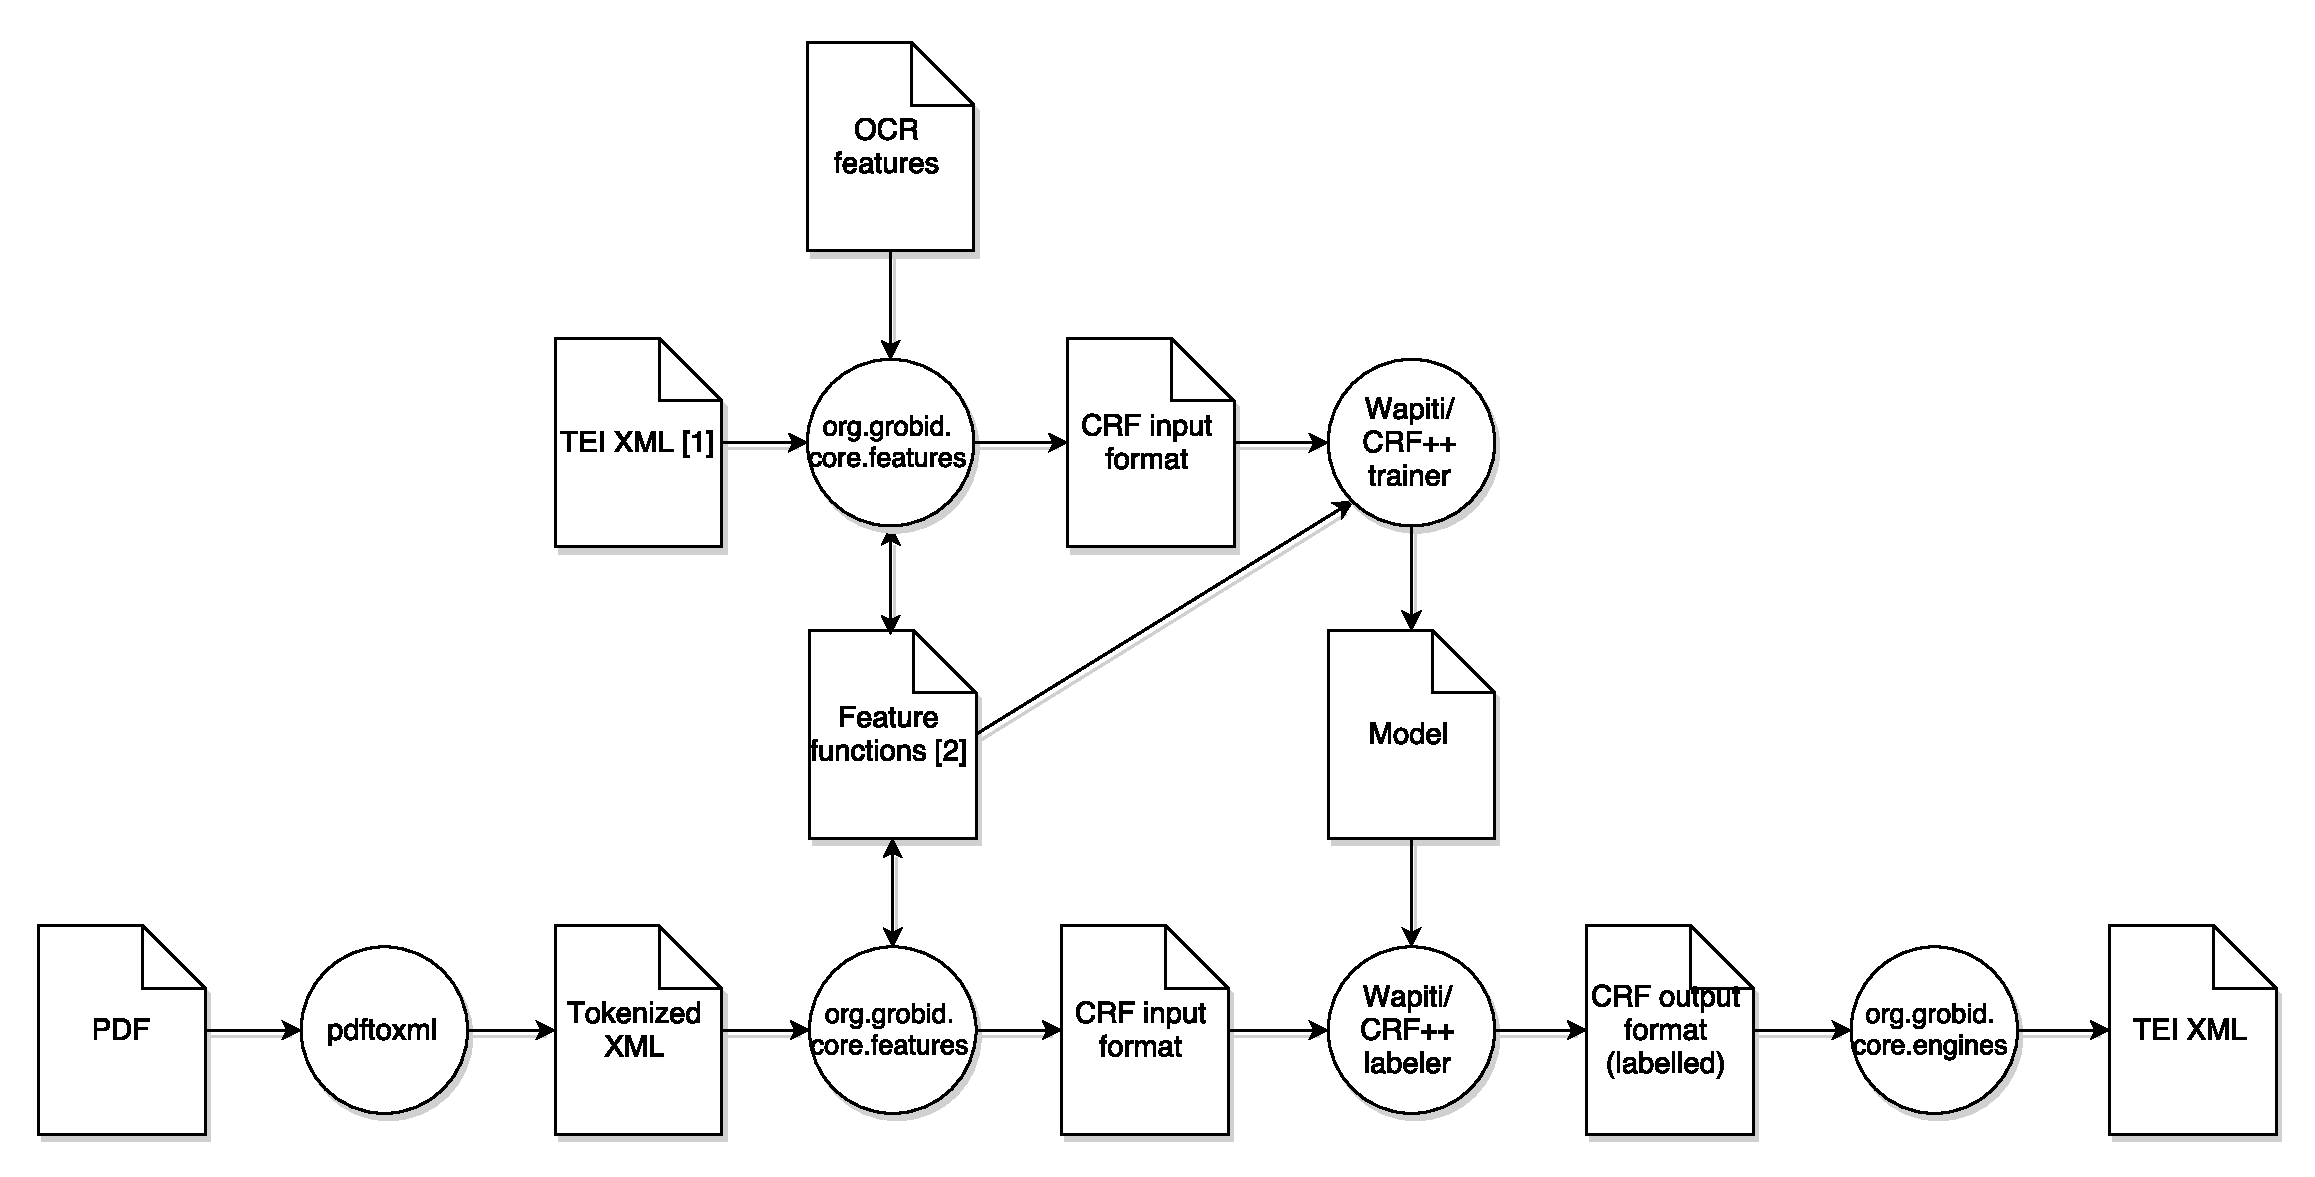
\includegraphics[width=6in]{Figures/grobid.pdf}
\caption{An Illustration of the interactions between Grobid and Wapiti for the two main functions of training and tagging.}
\label{fig:HMM}
\end{figure}

\begin{figure}[!ht]
\center
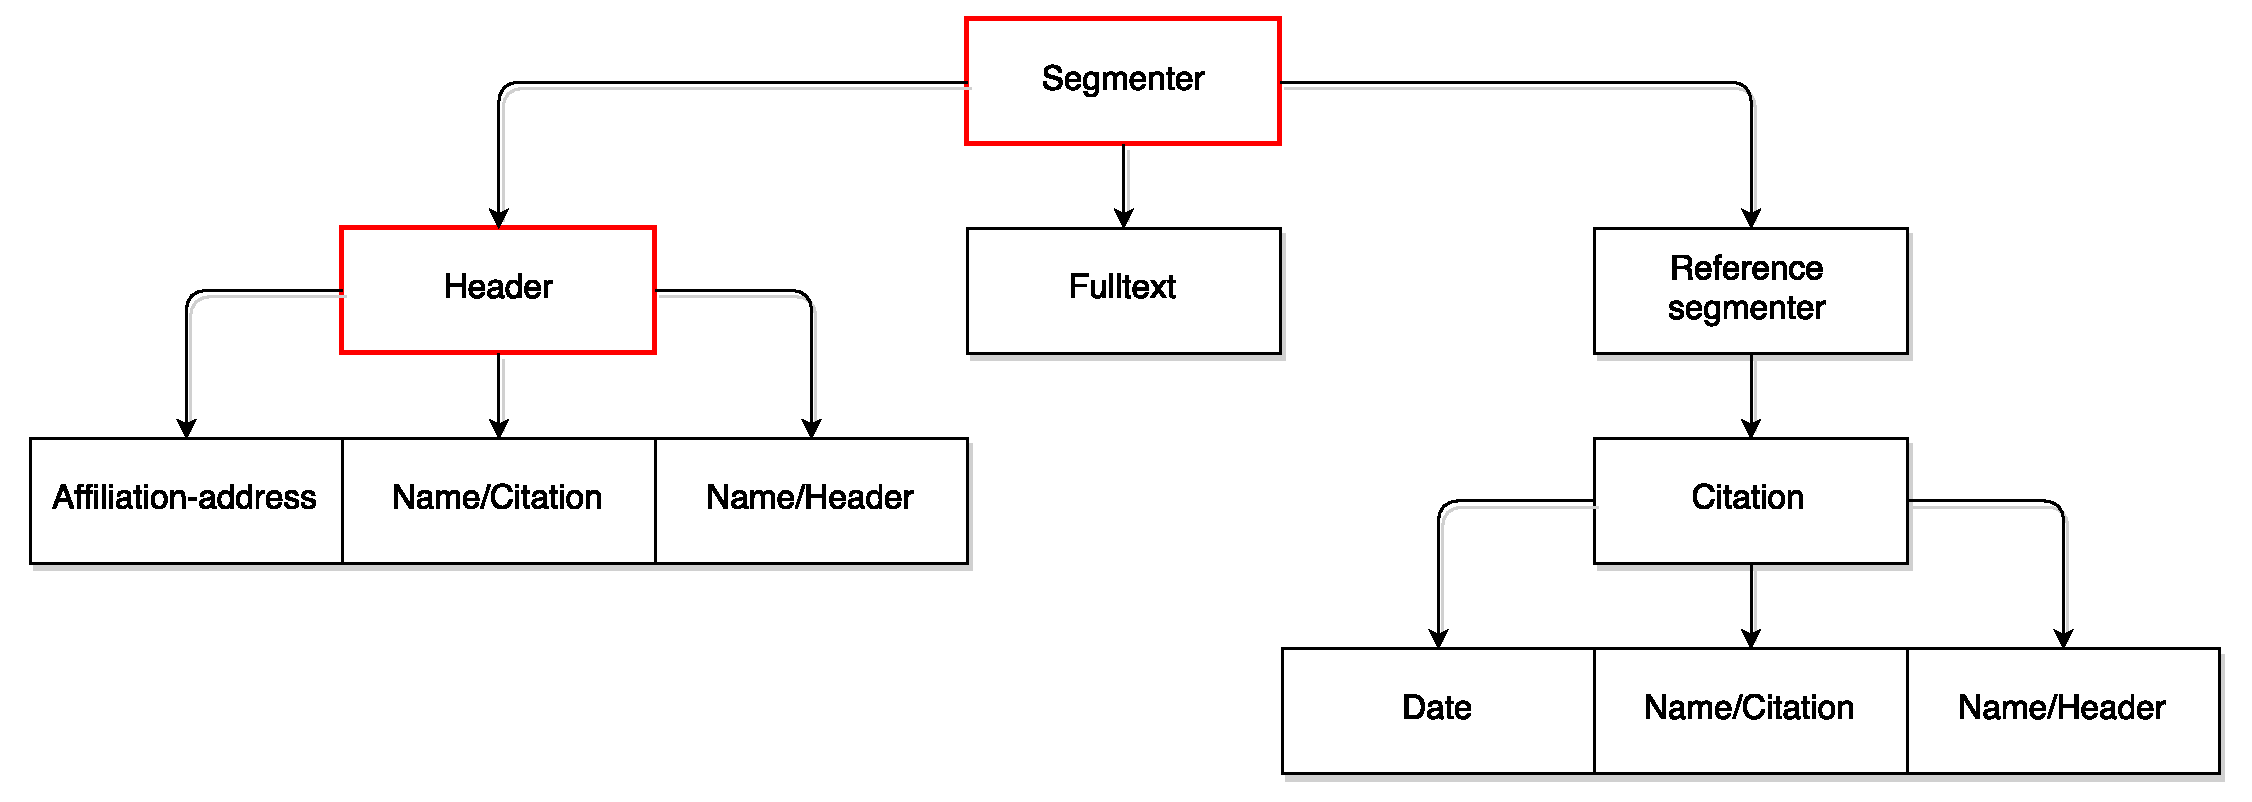
\includegraphics[width=6in]{Figures/cascade.pdf}
\caption{The models of Grobid are organised into a cascade, where each part of a document is classified in increasingly greater detail.}
\label{fig:HMM}
\end{figure}